%  Formatting the Paper  -------------------------------------------------------
\documentclass[a4paper,11pt]{report}

% adjust margins
\usepackage[right=1in,top=1in,left=1in,bottom=1in]{geometry}


%  Packages Used  --------------------------------------------------------------
\usepackage[english]{babel}
\usepackage[pdftex]{color,graphicx}   % graphics (images)
\usepackage{amsmath}
\usepackage{subfig}
\usepackage{graphicx}

%  Start the Paper  ------------------------------------------------------------
% define the title
\title{Project 2B - Particle Filters}
\author{Qandeel Sajid and Tina Nye}
\begin{document}
\maketitle

% insert the table of contents
\newpage
\tableofcontents
\newpage

\section{Project Description}

The project is on implementing a particle filter algorithm to locate the position and orientation of a moving agent using a known map of the environment and sensing input. The particle filter algorithm is a sampling-based approach that estimates a Bayesian model. There are four parts to this project. First, the students are expected to make a user interface that allows the user to make a map and chose the path the agent follows. For the the second and third parts, the program implemented by user should output observations by the agents with random noise and then reconstruct the agent's path based on these observations. The last part of the project combines everything to implement a particle filter.

\section{Discussion and Experiments}
	\subsection{Interface}
	The first part of the project is to implement an interface for users. This interface is meant to represent the continuous world of the agent. The world is filled with randomly generated landmarks with the quantity depending on the user's input. The landmarks are represented as black dots. Then, the interface allows the user to chose the path of the agent by clicking in desired destinations. The agent will move to the points one by one. Figure~\ref{fig:interface_agent} shows a sample interface in which the agent is moving towards the next user chosen destination. The red line represents the path of the agent. The robot is capable of moving at constant velocity (2 pixels per second) and rotate at constant rotational velocity (1 radian per second).
	
	%% show the graph image
	\begin{figure}[h!]
	  \centering
	    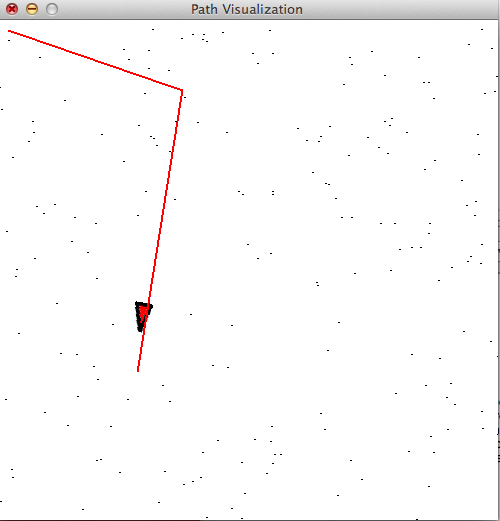
\includegraphics[width=.5\textwidth]{images/interface_agent.png}
	  \caption{Sample of the user interface.}
	  \label{fig:interface_agent}
	\end{figure}
	%%%%%%
	
	The map and the path are outputted by the program as map.txt and path.txt files. The path file contains the x, y and $\theta$ values at each state. Figures ~\ref{fig:map_simple} and ~\ref{fig:map_star} show the two maps and paths that are used for many of the later experiments.

	%% show the graph image
	\begin{figure}
	\centering
	\subfloat[Simple map/path.]{\label{fig:map_simple} 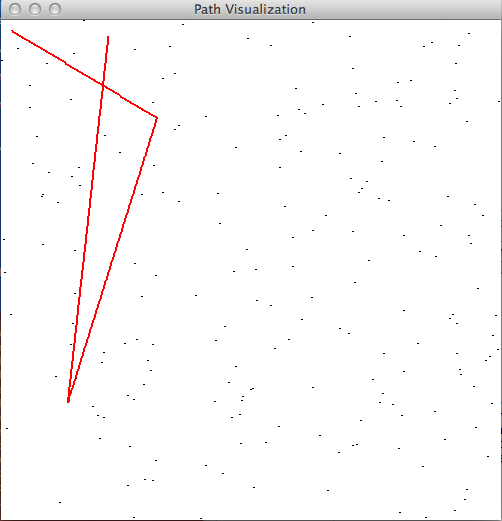
\includegraphics[width=.4\textwidth]{images/map_simple.png}}
	\subfloat[Star map/path.]{\label{fig:map_star} 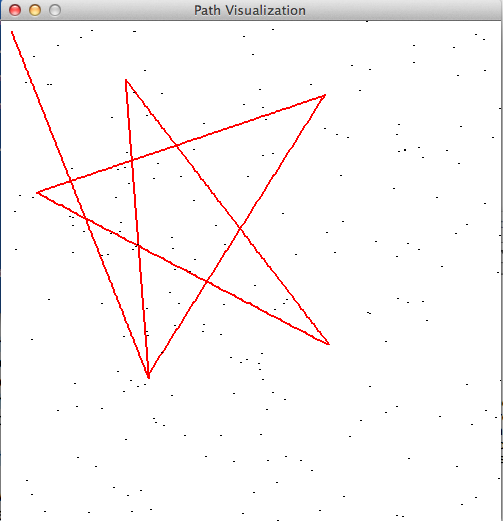
\includegraphics[width=.4\textwidth]{images/map_star.png}}
	\caption{Sample maps/paths.}
	\label{fig:simple_sensing}
	\end{figure}
	%%%%%%
	
	\subsection{Observations}
	Once the user has provided the "ground truth," which is the actual path the agent takes, sensing input can be simulated. At each step in the agent's path, the agent can sense: a) the displacement from the previous [x,y] location, b) the agent's change in orientation, c) the landmarks within the visibility range of the robot, d) for each landmark, the relative angle between the robot's orientation and the direction of the landmark. If there is no noise, the sensing input can be computed using the equations in Fig.~\ref{fig:equations}
	
	%% show the graph image
	\begin{figure}[h!]
	  \centering
	    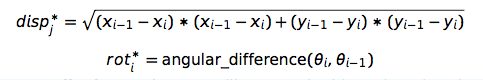
\includegraphics[width=.7\textwidth]{images/equations.png}
	  \caption{Basic methods of finding displacement and change in orientation.}
	  \label{fig:equations}
	\end{figure}
	%%%%%%
	
	For this program, five different sensing files are outputted using a visibility range of 40 pixels. The first file has no noise so the sensing input is computed using the equations above. One file has Gaussian noise in the displacement with the standard divination of 0.25, another has noise in the rotation measurement of standard deviation 0.01 radians. The fourth file combines the above two, and the fifth uses standard deviations of 0.5 for pixel displacement and 0.03 radians for rotations. The mean in all the experiments is 0.
	

	
	The program then uses the sensing files and the map to visualize the path generated by the sensing input. To reconstruct  the path, the equation shown in Fig.~\ref{fig:equation_2} is used. 
	%% show the equation
	\begin{figure}[h!]
	  \centering
	    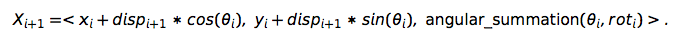
\includegraphics[width=1\textwidth]{images/equation_2.png}
	  \caption{Equation for reconstructing the agents position at x$_{i+1}$,  y$_{i+1}$ and  $\theta_{i+1}$ using  x$_{i}$, y$_{i}$ and $\theta_{i}$.}
	  \label{fig:equation_2}
	\end{figure}
	%%%%%%
		
		%% show image
	\begin{figure}[t!]
	\centering
	\subfloat[No noise.]{\label{fig:simple_1} 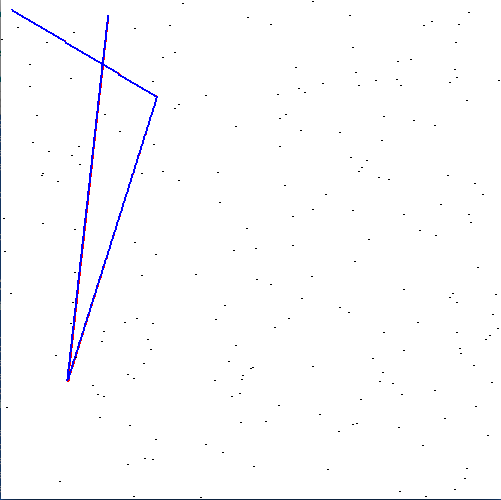
\includegraphics[width=.3\textwidth]{images/simple_1.png}}
	\subfloat[Standard deviation=0.25 pixels.]{\label{fig:simple_2} 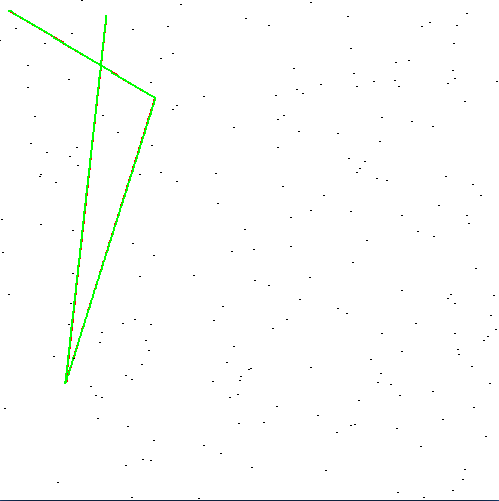
\includegraphics[width=.3\textwidth]{images/simple_2.png}}
	\subfloat[Standard deviation=0.01 radians.]{\label{fig:simple_3} 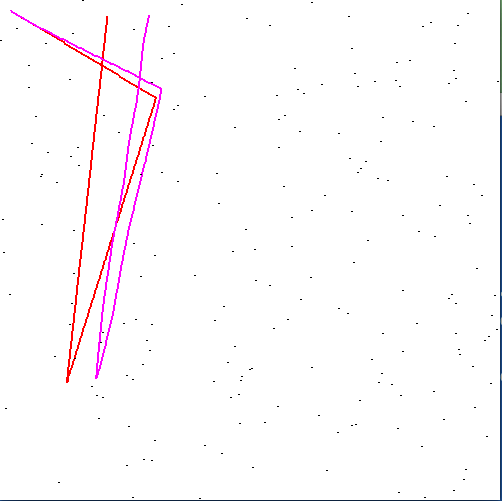
\includegraphics[width=.3\textwidth]{images/simple_3.png}}
	\\
	\subfloat[Standard deviation=0.25 pixels and 0.01 radians.]{\label{fig:simple_4} 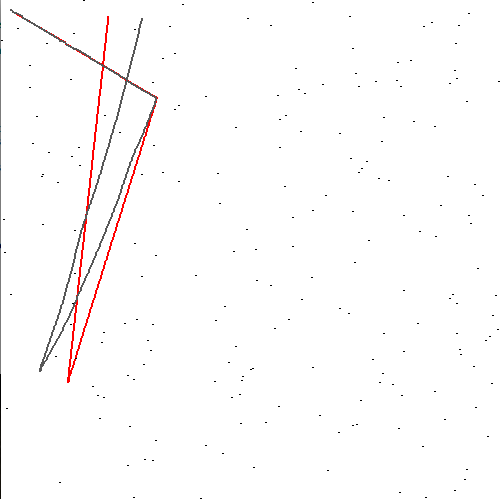
\includegraphics[width=.3\textwidth]{images/simple_4.png}}
	\subfloat[Standard deviation=0.5 pixels and 0.03 radians.]{\label{fig:simple_5} 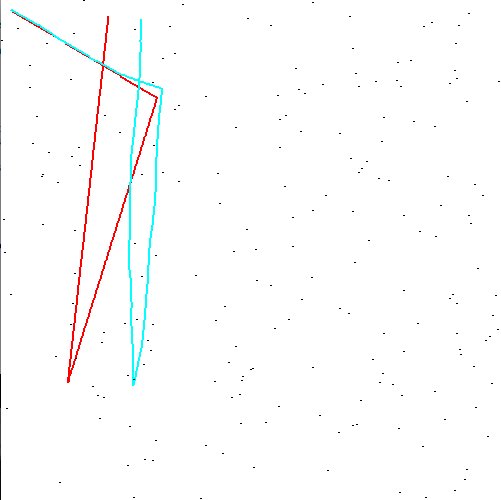
\includegraphics[width=.3\textwidth]{images/simple_5.png}}
	\caption{Sensing files for the simple map/path.}
	\label{fig:simple_sensing}
	\end{figure}
	%%%%%%
	After reconstructing the path from the sensing files, they are compared to the "ground truth." Figure~\ref{fig:simple_sensing} shows the paths generated from reconstructing the sensing inputs for the simple path. In all of the images, the "ground truth" is represented in red. For the comparison with the no noise input,~\ref{fig:simple_1} shows that the reconstructed path mostly overshadows the "ground truth," the same is true from the sensing input with noise added only to the displacement.~\ref{fig:simple_3} -~\ref{fig:simple_5} show the reconstructed path deviates from the "ground truth" as noise is added to the orientation. 
	

	
	%% show image
	\begin{figure}[t!]
	\centering
	\subfloat[No noise.]{\label{fig:star_1} 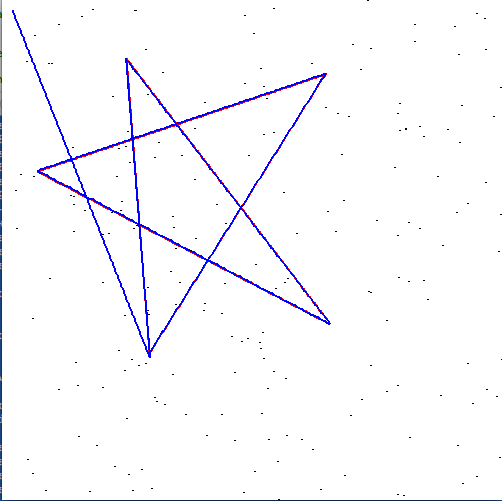
\includegraphics[width=.3\textwidth]{images/star_1.png}}
	\subfloat[Standard deviation=0.25 pixels.]{\label{fig:star_2} 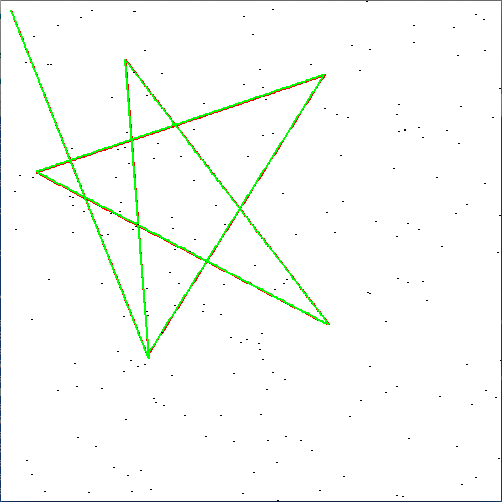
\includegraphics[width=.3\textwidth]{images/star_2.png}}
	\subfloat[Standard deviation=0.01 radians.]{\label{fig:star_3} 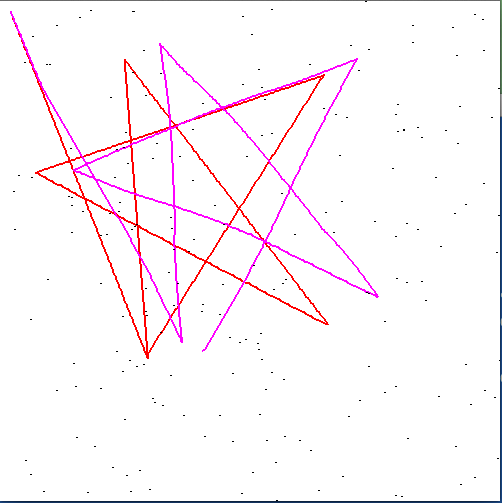
\includegraphics[width=.3\textwidth]{images/star_3.png}}
	\\
	\subfloat[Standard deviation=0.25 pixels and 0.01 radians.]{\label{fig:star_4} 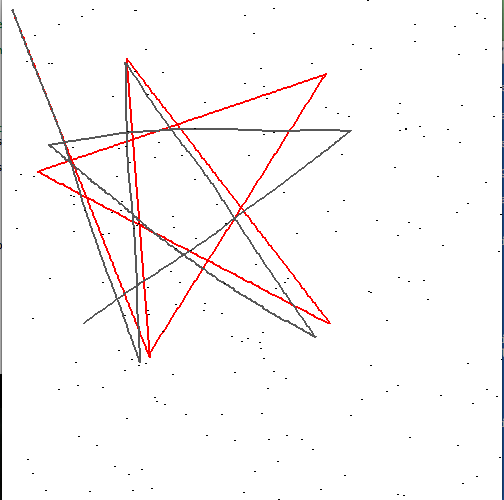
\includegraphics[width=.3\textwidth]{images/star_4.png}}
	\subfloat[Standard deviation=0.5 pixels and 0.03 radians.]{\label{fig:star_5} 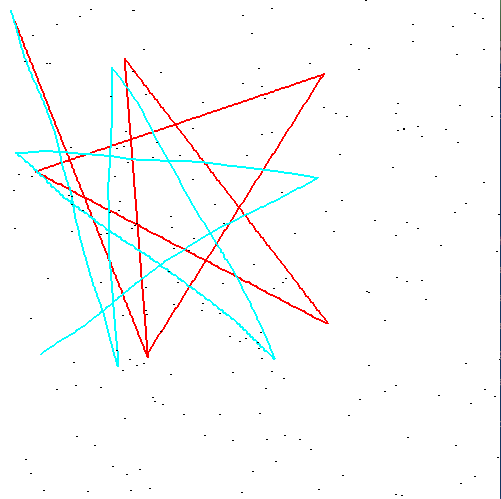
\includegraphics[width=.3\textwidth]{images/star_5.png}}
	\caption{Sensing files for the star map/path.}
	\label{fig:star_sensing}
	\end{figure}
	%%%%%%
	
	Simpler comparisons are done for the map with the star shaped path. These comparisons are shown in Fig.~\ref{fig:star_sensing}. The results are similar to that of the simple path in Fig.~\ref{fig:simple_sensing}.
	
		\begin {table}[h]\small
		\centering
		\begin{tabular*}{0.66\textwidth}[left]{|c|c|c|c|c|}
		\hline
		  Sensing file & \multicolumn{2}{|c|}{Simple PS} & \multicolumn{2}{|c|}{StarPS}\\
		  \hline
		  Errors & Displacement & Angle & Displacement & Angle\\
		  \hline
		  1 & 2.23e-12 & 8.62e-14  & 2.47e-12 & 9.94e-14 \\
		  2 & 0.041 & 8.62e-14 & .042 & 9.94e-14\\
		  3 & 2.23e-12 & 2.71 & 2.47e-12 & 3.71  \\
		  4 & 0.040 & 6.50 & 0.039 & 25.46\\
		  5 & 0.055 & 7.50 & 0.057 & 54.69 \\
		  \hline
		
		\end{tabular*}
		    \caption{{\small Average error in the displacement and orientation.}}
		\end{table}
		
		The Table 1 shows the average error in displacement and orientation of the sensed paths and "ground truth." The results in the table correspond to the visualization of reconstructed paths. 
		
	\subsection{Particle Filter}
		
		\begin{figure}[t!]
		\centering
		\subfloat[No noise. 150 particles, with average error 1.50 pixels.]{\label{fig:simple_150_1} 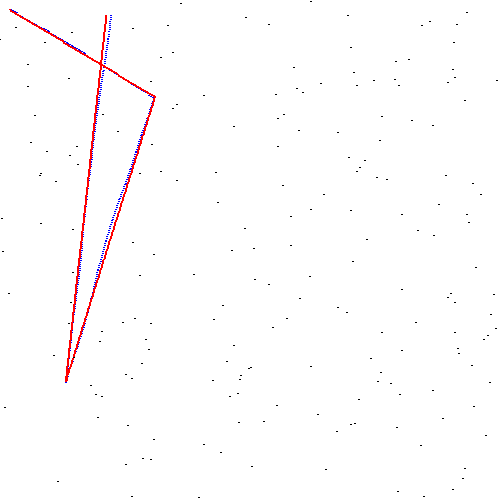
\includegraphics[width=.3\textwidth]{images/simple_150_1.png}}
		\subfloat[Standard deviation=0.25 pixels. 150 particles, with average error 1.54 pixels.]{\label{fig:simple_150_2} 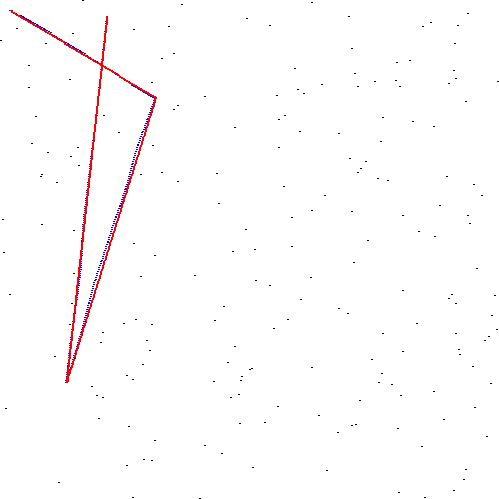
\includegraphics[width=.3\textwidth]{images/simple_150_2.png}}
		\subfloat[Standard deviation=0.01 radians. 150 particles, with average error 1.43 pixels.]{\label{fig:simple_150_3} 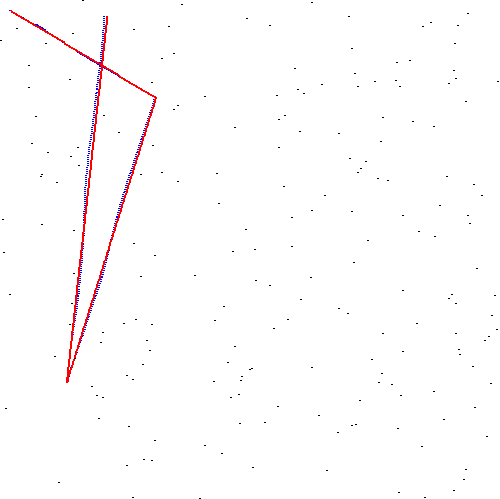
\includegraphics[width=.3\textwidth]{images/simple_150_3.png}}
			\\
		\subfloat[Standard deviation=0.25 pixels and 0.01 radians. 150 particles, with average error 1.94 pixels.]{\label{fig:simple_150_4} 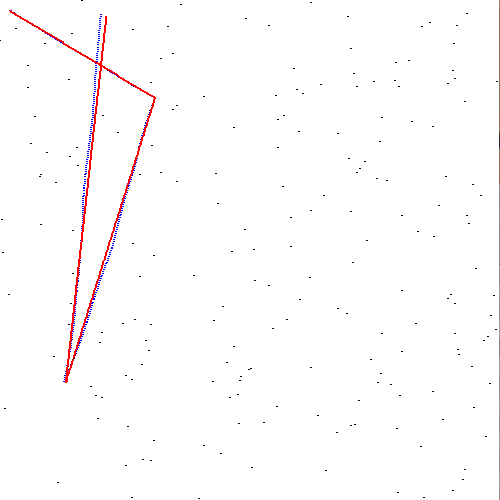
\includegraphics[width=.3\textwidth]{images/simple_150_4.png}}
		\subfloat[Standard deviation=0.5 pixels and 0.03 radians. 150 particles, with average error 9.90 pixels.]{\label{fig:simple_150_5} 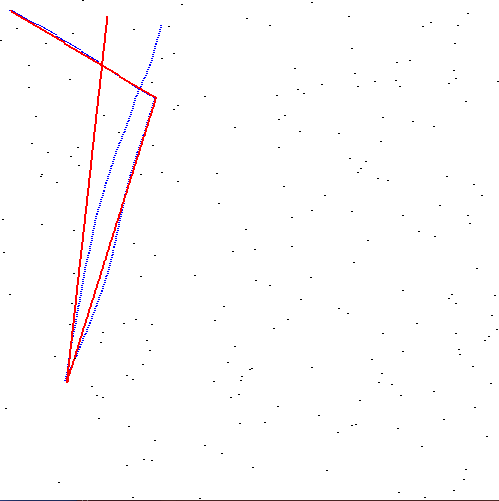
\includegraphics[width=.3\textwidth]{images/simple_150_5.png}}
		\caption{Execution of the particle filter on the simple map/path.}
		\label{fig:simple_with_diff_sensing}
		\end{figure}

		
	The particle filter algorithm implemented in this program is a sampling-based approach to solving the filtering problem in which the new belief distribution depends on the previous belief distribution. The transition model is defined using the sensing input as shown in Fig.~\ref{fig:equation_2} with some addition noise. The observation model uses a particles' location and orientation to determine the probability of  receiving the expected observations. For this program, the probability is found by comparing the landmarks the particle observes in its location to the evidence. The observation model takes the evidence landmarks and checks where the particle observes those landmarks. The number of evidence landmarks observed within 45 degrees of the angle relative to the agent that was actually observed over the total number of evidence landmarks it should observe is multiplied with the amount of evidence landmarks within 20 and 10 degrees of the actual evidence. If the particle observes all the evidence landmarks within 10 degrees of the actual evidence, it will have a weight of 1.0.
		
	Originally in the algorithm, a population of P particles are initialized to the prior belief distribution which is required for the problem. Then the transition model is applied to each particle. Each particle receives weights from the observation model which are used in the resampling process. During resampling, the particles with weight 0 are ignored unless if all the particles have a weight of 0. In this case, the new population is the same as the old. This process repeats until no sensing input is left.
	
	Figures~\ref{fig:simple_with_diff_sensing} and ~\ref{fig:star_with_diff_sensing} show the result of applying the particle filter using the five sensing model on the two maps. This test is done using 150 particles. In the figures the red represents the ground truth and the blue is the reconstructed path of the particle with the highest weight at the last iteration of the algorithm. As shown by the figures, most of the time the particles are capable of computing the ground truth with little error. The worse computations occur with the fifth sensing model (Figures~\ref{fig:star_150_5} and \ref{fig:simple_150_5}) which has more noise in its displacement and rotation. Due to the high noise levels, the observations generated by the fifth sensing model is usually inaccurate since the agent's path is significantly different from the ground truth causing it to observe different landmarks. 
	

		\begin{figure}[t!]
		\centering
		\subfloat[No noise. 150 particles, with average error 0.98 pixels.]{\label{fig:star_150_1} 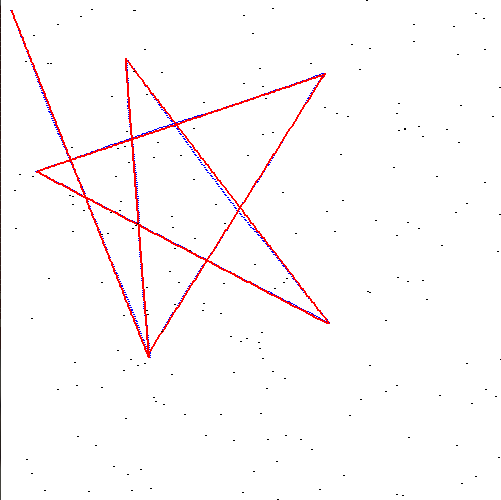
\includegraphics[width=.3\textwidth]{images/star_150_1.png}}
		\subfloat[Standard deviation=0.25 pixels. 150 particles, with average error 1.28 pixels.]{\label{fig:star_150_2} 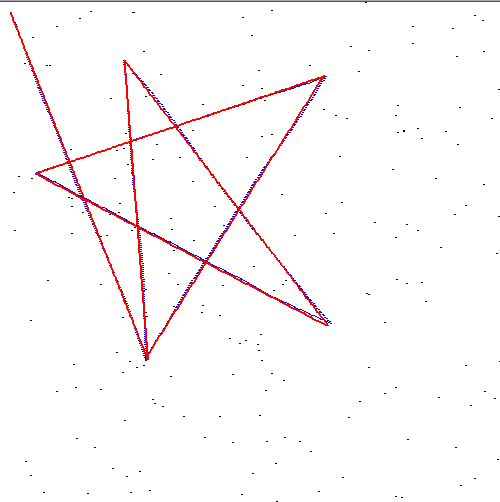
\includegraphics[width=.3\textwidth]{images/star_150_2.png}}
		\subfloat[Standard deviation=0.01 radians. 150 particles, with average error 1.24 pixels.]{\label{fig:star_150_3} 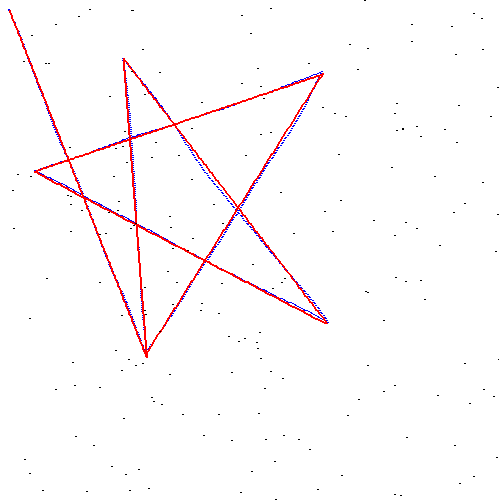
\includegraphics[width=.3\textwidth]{images/star_150_3.png}}
			\\
		\subfloat[Standard deviation=0.25 pixels and 0.01 radians. 150 particles, with average error 1.21 pixels.]{\label{fig:star_150_4} 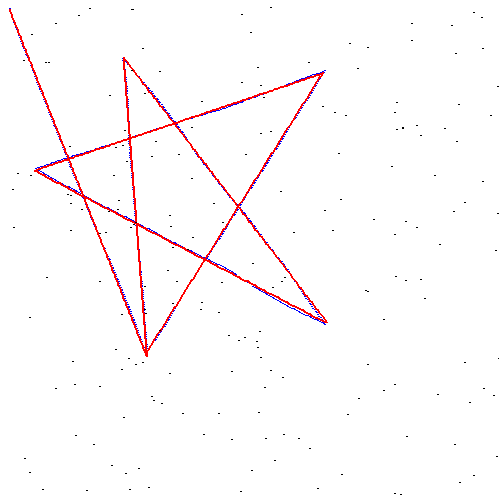
\includegraphics[width=.3\textwidth]{images/star_150_4.png}}
		\subfloat[Standard deviation=0.5 pixels and 0.03 radians. 150 particles, with average error 29.92 pixels.]{\label{fig:star_150_5} 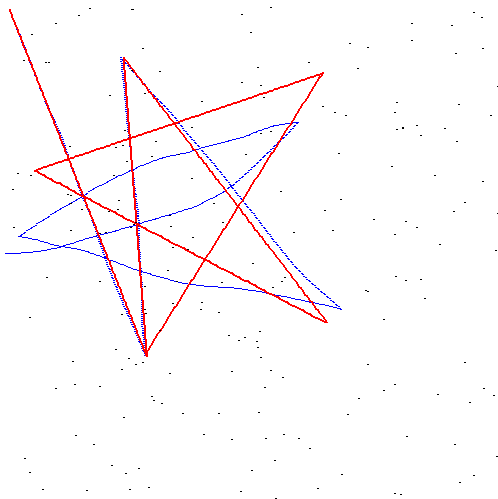
\includegraphics[width=.3\textwidth]{images/star_150_5.png}}
		\caption{Execution of the particle filter on the star map/path.}
		\label{fig:star_with_diff_sensing}
		\end{figure}
	
	\subsection{Implementation Details}
	The implementation of the program follows an object orientation approach using the following classes:
	
		State - class that contains the agent's x, y, $\theta$ configurations.
	
		Path - contains a list of State objects
	
		Observation - Each observation object contains the displacement, rotation, number of landmarks, landmark ids and rotation for each state. When the sensing input is loaded, a list of observation objects is used.
	
		Landmark - Each landmark object contains the id, and position of the landmark. For all the landmarks in the map, a list of landmark objects is used.
	
		Particle - Each particle object contains the path, weight, index, and average error of the path for that particle.
	
		Particle Filter - The particle filter object contains a list of particles and the observations being used. It also contains the functions required for the implementation of the particle filter. Some of those functions include the transition model and the observation model. The particle filter is executed by calling the algorithm function.
		
	There is no class for the map since it only uses the landmarks list. One program is implemented for this project. What the program does depends on the input provided. The program was also implemented using Python.
		
		

	\subsection{Experiments}


		\subsubsection{Results}
		Figures ~\ref{fig:simple_sensing_results} and ~\ref{fig:star_sensing_results} show the results of using the particle filter on a problem with 200 landmarks, and a visibility range of 40. In the figures, the "ground truth" is represented in red, and the path found by the particle filter in blue. As shown by the results, as the number of particles increase, the average error decreases leading to a better approximation of the "ground truth." Two more test are discussed later in the paper.
		
			\begin{figure}[t!]
			\centering
			\subfloat[20 particles, with average error 1.97 pixels.]{\label{fig:simple_1_p} 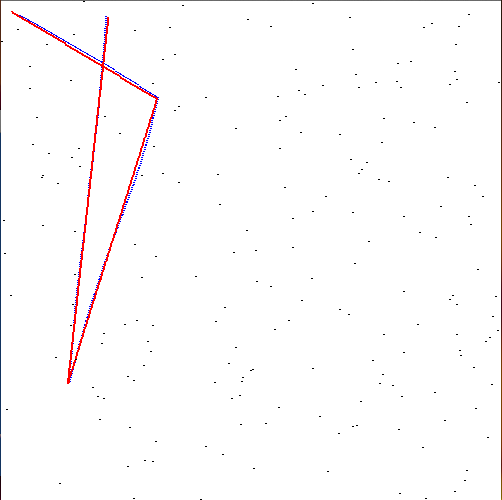
\includegraphics[width=.3\textwidth]{images/simple_40v_20p.png}}
			\subfloat[40 particles, with average error 1.67 pixels.]{\label{fig:simple_2_p} 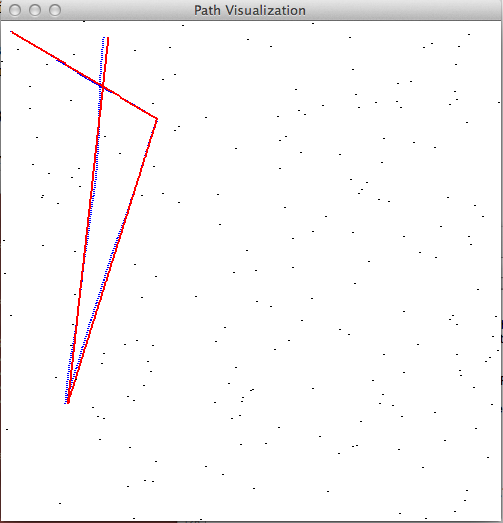
\includegraphics[width=.3\textwidth]{images/simple_40v_40p.png}}
			\subfloat[60 particles, with average error 1.23 pixels.]{\label{fig:simple_3_p} 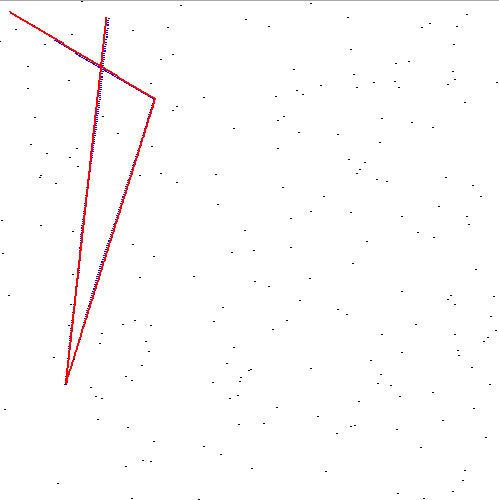
\includegraphics[width=.3\textwidth]{images/simple_40v_60p.png}}
			\\
			\subfloat[80 particles, with average error 1.09 pixels.]{\label{fig:simple_4_p} 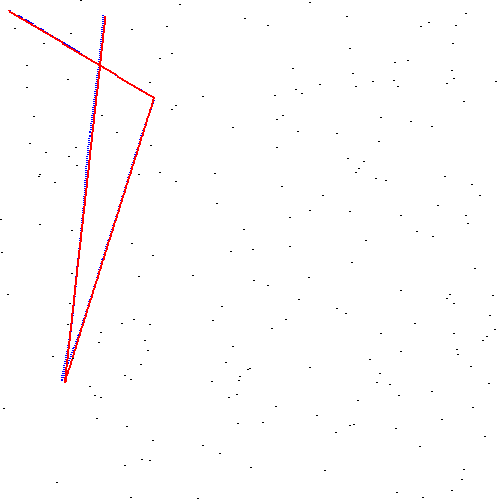
\includegraphics[width=.3\textwidth]{images/simple_40v_80p.png}}
			\subfloat[100 particles, with average error 0.99 pixels.]{\label{fig:simple_5_p} 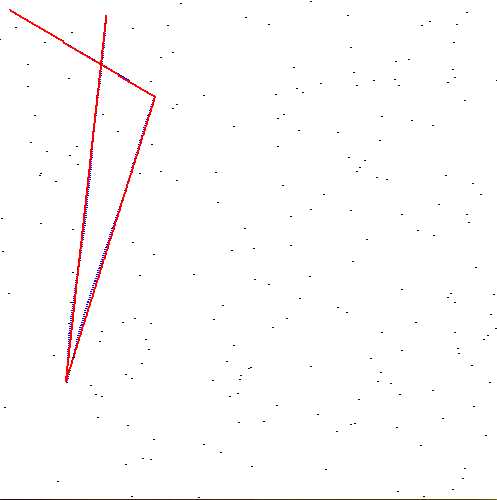
\includegraphics[width=.3\textwidth]{images/simple_40v_100p.png}}
			\caption{Execution of the particle filter on the simple map/path.}
			\label{fig:simple_sensing_results}
			\end{figure}
			
			
			\begin{figure}[t!]
			\centering
			\subfloat[20 particles, with average error 1.91 pixels.]{\label{fig:simple_1_s} 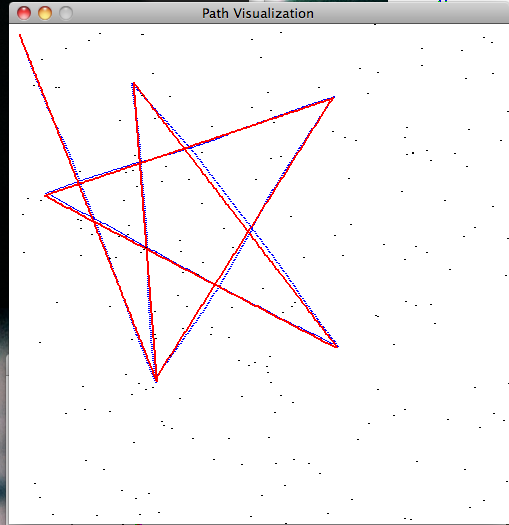
\includegraphics[width=.3\textwidth]{images/star_40v_20p.png}}
			\subfloat[40 particles, with average error 1.73 pixels.]{\label{fig:simple_2_s} 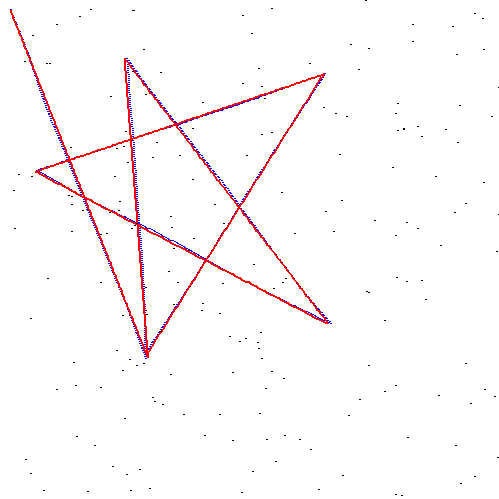
\includegraphics[width=.3\textwidth]{images/star_40v_40p.png}}
			\subfloat[60 particles, with average error 1.64 pixels.]{\label{fig:simple_3_s} 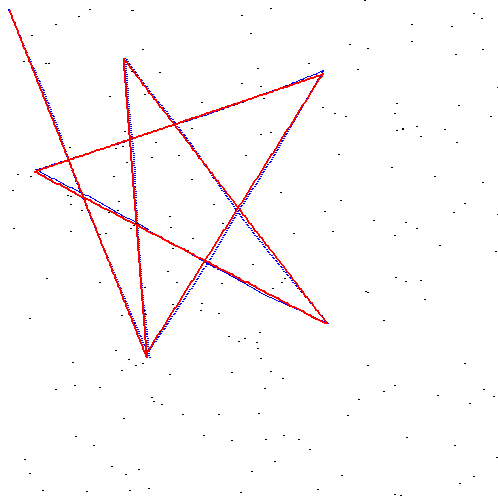
\includegraphics[width=.3\textwidth]{images/star_40v_60p.png}}
			\\
			\subfloat[80 particles, with average error 1.14 pixels.]{\label{fig:simple_4_s} 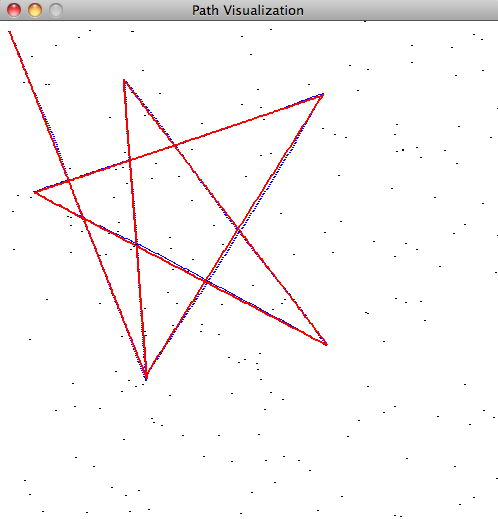
\includegraphics[width=.3\textwidth]{images/star_40v_80p.png}}
			\subfloat[Standard deviation=0.5 pixels and 1.01 radians.]{\label{fig:simple_5_s} 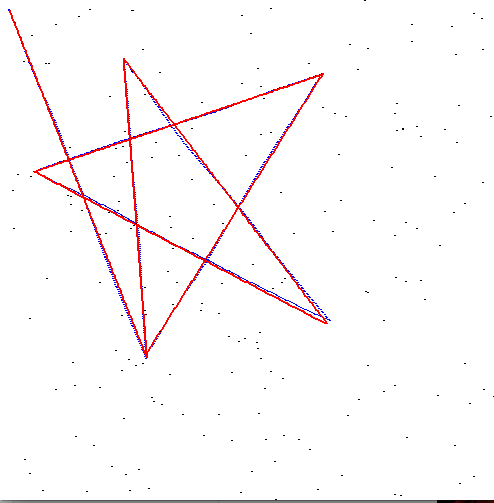
\includegraphics[width=.3\textwidth]{images/star_40v_100p.png}}
			\caption{Sensing files for the simple map/path.}
			\label{fig:star_sensing_results}
			\end{figure}
			

		\subsubsection{Changing Visibility Range}
		One of the experiments done in the project is testing the effect of different visibility range. The tests were done by changing the visibility range but keeping the number of particles to 60, and the landmarks to 200 on the simple path. Although it would be expected that as the visibility range increases the average error decreases since the agent will be able to compare with more evidence, the results contradict this. 
		
			\begin {table}[h]\small
			\centering
			\begin{tabular*}{0.278\textwidth}[left]{|c|c|c|c|c|}
				\hline
				  Visibility & Average Error\\
				  \hline
				  20 & 2.47 \\
				  40 & 1.23 \\
				  60 & 2.56 \\
				  80 & 2.47 \\
				  100 & 1.46 \\
				  \hline
				
				\end{tabular*}
				    \caption{{\small Average error as the visibility range changes}}
				\end{table}
				
		The results in Table 2 show that after the error decreases for the visibility range of 40, it increases again for the range of 60. Then, the error drops again. It is possible that choosing only 60 particles might have been low causing the results to behave somewhat randomly.
		
		\subsubsection{Changing Density of Landmarks}
		The second experiment is testing the effect of changing the density of the landmarks. For this, the visibility range is left at 40 and the number of particles at 60 for the simple path example. As shown by the results in Table 3, the average error decreases as the number of landmarks increase. This is accurate since the observation model is based on the visible landmarks. With more landmarks, the agent senses more and the particles will have to try and match that many evidence landmarks.
			\begin {table}[h]\small
			\centering
			\begin{tabular*}{0.3\textwidth}[left]{|c|c|c|c|c|}
				\hline
				  Landmarks & Average Error\\
				  \hline
				  100 & 2.42 \\
				  200 & 1.23 \\
				  300 &  1.09\\
				  400 &  0.94\\
				  500 &  0.79\\
				  \hline
				
				\end{tabular*}
				    \caption{{\small Average error as the number of landmarks change.}}
				\end{table}
				
		\subsubsection{In which cases does the algorithm work better?}
		Better results are computed as the number of particles increase. With more particles, the resampling is better since it chooses the best out of a large variety of particles. The algorithm also works better when it has more observations.
		
		\subsubsection{Ideas on how the algorithm can be improved?}
		The worst part of the particle filtering algorithms is that it requires many particles to compute the result accurately. Increasing the number of particles results in many computations which can take a long time. Another problem with the particle filter is that it might not observe anything or every particle has the same weight. In this case there in no point in resampling since the no new information was gained. To fix this problem it would likely be better to not sample from the current batch of particles and increase the noise for the next state. The transition and observation models would increase the noise every time resampling does not occur in the previous state.
		
		The simplest option is to ensure there are plenty of observations/evidence at each state. It can also add distance from the origin as evidence to keep the particle wondering too far from the path.
		
		\subsubsection{What if the environment contained obstacles?}
		If the environment contains obstacles, there is no point in changing the transition model. The model tries to reconstruct the next state plus some noise. It would be inefficient to check if the additional noise leads to collisions with obstacles. Instead, it would be better to improve the observation model. Currently, the observation model judges the accuracy of the particles location based on the evidence landmarks. With obstacles, they also become part of the evidence. Considering the particles have a known map, it should be able to observe if they are about to collide with obstacles give the weight of that state a 0. If in this case all of the particles result in 0 weights, it's better to add more random noise in the transition.
			
\end{document}
